\section{Bison}

What syntax is valid or not is defined by the grammar. A syntactic analysis must:
\begin{itemize}
    \item Identify grammar structures.
    \item Verify syntactic correctness.
    \item Build a (possibly unique) derivation tree for the input.
\end{itemize}
Syntactic analysis does not determine the meaning of the input. That is the task of the semantic analysis. The syntactic analysis is performed over a stream of
terminal symbols. Non-terminal symbols are only generated through reduction of grammar rules. 

Bison is the standard tool to generate LR parsers, and it is designed to work seamlessly together with flex. It is a generated parser that uses LALR(1) methodology.
The generated parser implements a table driven push-down automaton:
\begin{itemize}
    \item The pilot automaton is described as finite state automaton.
    \item The parsing stack is used to keep the parser state at runtime.
    \item Acts as a typical shift-reduce parser.
\end{itemize}

\subsection*{File format}
A bison file is structured in four sections:
\begin{itemize}
    \item Prologue: useful place where to put header file inclusions, variable declarations. 
    \item Definitions: definition of tokens, operator precedence, non-terminal types. 
    \item Rules: grammar rules. 
    \item User code: C code (generally helper functions), specified in BNF notation.
\end{itemize}
Different syntactic elements can be defined using $\%$token. In the generated parser each token is assigned a number; in this way you can use them in the lexer. 

Just like Flex, Bison allows to specify semantic actions in grammar rules. A semantic action is a conventional C code block and can be specified at the end of 
each rule alternative. Semantic actions are executed when the rule they are associated with has been completely recognized. The consequence is that the order of 
execution of the actions is bottom-up. You can also place semantic actions in the middle of a rule. Internally bison normalizes the grammar in order to have only
end-of-rule actions, and this can introduce ambiguities

$\%$union declaration specifies the entire collection of possible data types. Type specification for terminals (tokens) in the token declaration. Type 
specification for non-terminals in special $\%$type declarations. The semantic value of each grammar symbol in a production is a variable called $\$i$, where 
$i$ is the position of the symbol. $\$\$$ corresponds to the semantic value of the rule itself. 

\subsection*{Interface and integration}
Bison generates a parser that is a C file with suffix .tab.c and an header with declarations with suffix .tab.h. The main parsing function is "int yyparse(void)". 
For reading tokens the parser uses the same "yylex()" function that flex-generated scanners provide. 

To integrate Flex and Bison we have to: 
\begin{enumerate}
    \item Include the *.tab.h header generated by Bison. 
    \item In the semantic actions: assign the semantic value of the token (if any) to the correct member of the yylval variable, and return the token identifiers 
        declared in Bison. 
    \item Declare and implement the main() function. 
    \item Generate the flex scanner by invoking Flex. 
    \item Generate the Bison parser by invoking Bison. 
    \item Compile the C files produced by Bison and Flex together. 
\end{enumerate}
The first two points are for Flex and the third one is for Bison source code. Graphically we have the following schema. 
\begin{figure}[H]
    \centering
    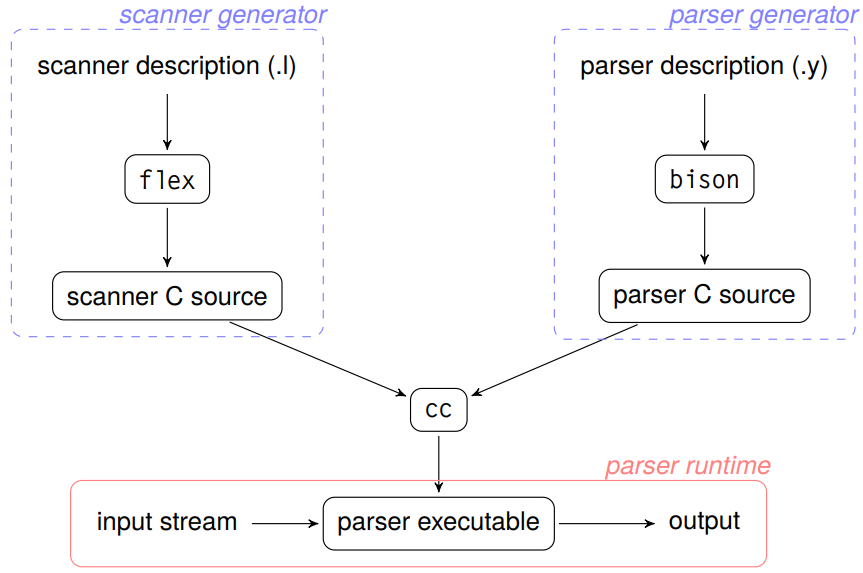
\includegraphics[width=0.8\linewidth]{images/flbi.png}
\end{figure}